\section{Transversely Polarized Target}

Measurements of the transverse target single spin asymmetry (SSA) for 
different final state particles in semi-inclusive and exclusive hard 
processes, including photon deeply virtual Compton scattering (DVCS), and
pseudoscalar and vector meson production in a wide range of different 
kinematic variables are a critical part of the {\tt CLAS12} physics program.
Our preliminary studies show that it is technically possible to run a 
polarized target with {\tt CLAS12}.  Two main options for a transversely 
polarized target are currently under consideration:

\begin{itemize}
\item Standard transverse target with 4.2~T field;
\item HD target.
\end{itemize}

\subsection{Standard Transversely Polarized Target}

For {\tt CLAS12} operation with the standard transversely polarized
target, the solenoid magnet and central detector will be removed 
and replaced by a stand-alone polarized target, similar to the existing 
polarized target used in electron scattering experiments.  As the magnetic 
field orientation is transverse to the beam direction, the electron beam 
will be deflected vertically. This will be compensated for by installing a 
magnetic chicane system upstream of the target so that the beam after the
target is again in the horizontal plane.  Special care is needed for 
shielding of the electromagnetic background, especially M{\o}ller electrons.
Note that the chicane system is necessary for transverse target operation,
and has to be robust enough to allow the beam to go through the center of 
the target and restored afterwards to go into the beam dump.

%%%%%%%%%%%%%%%%%%%%%%%%%%%%%%%%%%%%%%%%%%%%%%%%%%%%%%%%%%%%%%%%%%%%%%%%%%
\begin{figure}
\begin{center}
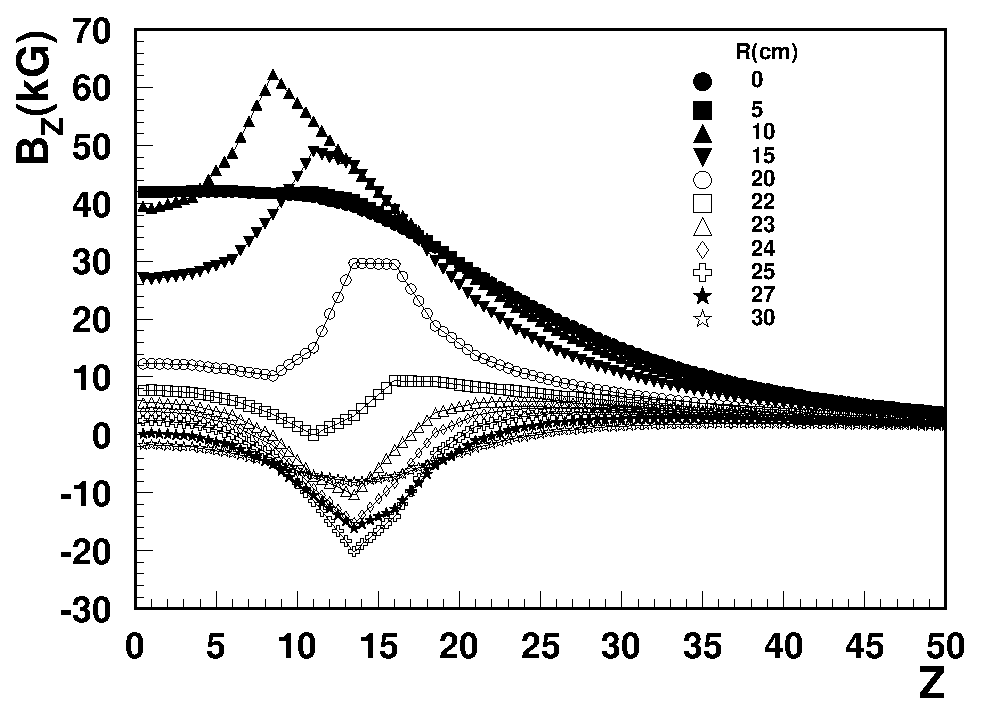
\epsfig{file=solfield.eps,width=14.0cm,height=8cm}
\vskip -0.2cm
\caption{\small{Transverse target magnetic field distribution in terms of
$B_z$ (kG) vs. $z$-coordinate (cm) for different radial distances.}}
\label{fig:solfield}
\end{center}
\end{figure}
%%%%%%%%%%%%%%%%%%%%%%%%%%%%%%%%%%%%%%%%%%%%%%%%%%%%%%%%%%%%%%%%%%%%%%%%%%

The basis for the design of a transversely polarized target is the 5~T 
magnet, which has been used very successfully in SLAC and JLab, along 
with a 1~K $^4$He evaporation refrigerator. The 5~T magnet was optimized 
for scattering with longitudinal polarization, but allowed a reasonable 
aperture for scattering with a transverse field.  This mode was used at 
both SLAC and JLab.  A similar magnet was built and operated successfully
with {\tt CLAS} in Hall B; modifications to the design were mandated by 
the magnet having to be supported inside {\tt CLAS}, and it could not be 
configured to operate with a magnetic field transverse to the electron beam. 
Both magnets were designed and built by Oxford Instruments, and through a 
cooperative effort with JLab and the University of Virginia, Oxford 
Instruments produced an optimized design for a high-field transverse magnet 
to be used in {\tt CLAS} for the 6-GeV program.  However, the target concept 
is such that it can be operated with {\tt CLAS12} as well.
 
The target will have a warm bore for the target cryostat that also allows 
detection of slow protons in specially designed magnetic field insensitive 
detectors located around the target cryostat. The target field map is shown 
in Fig.~\ref{fig:solfield}.  The magnet specifications are listed in 
Table~\ref{mag_parms}.

%%%%%%%%%%%%%%%%%%%%%%%%%%%%%%%%%%%%%%%%%%%%%%%%%%%%%%%%%%%%%%%%%%%%%%%%%%
\begin{table}[htbp]
\begin{center}
\begin{tabular}{|l|l|} \hline 
Central Field & 4.2~T at 4.2~K \\ \hline
Homogeneity   & 1 part in 10$^4$ over a 15~mm DSV (diameter spherical vol.) \\
              & 3 parts in 10$^4$ over a 25~mm DSV \\ \hline
Cold vertical access & 100~mm (helium temperature) \\
(for target access)  &                             \\ \hline
Bore access   & $\pm$35$^\circ$ onto a 25-mm diameter sphere. \\
              & Removable room temperature re-entrant cones on axis to \\
              & within 12~cm of central field position. \\ \hline
Split access  & Vertical: $\pm$35$^\circ$ onto 25-mm diameter sphere. \\
              & Horizontal: $\pm$22.5$^\circ$ onto a point. \\ \hline
\end{tabular}
\end{center}
\caption{\small{Listing of polarized target magnet parameters.}}
\label{mag_parms}
\end{table} 
%%%%%%%%%%%%%%%%%%%%%%%%%%%%%%%%%%%%%%%%%%%%%%%%%%%%%%%%%%%%%%%%%%%%%%%%%%

The refrigerator is vertical and will be very similar to that used in the
UVA/SLAC/JLab system with the target samples easily inserted and removed. The
target can operate in a beam of up to 100~nA, but it will be much less in
{\tt CLAS12}. Initial ammonia polarizations give $\pm$95\% for protons and 
38\% to 48\% for deuterons. The target is polarized continuously by applying
microwaves, and the most important process affecting the polarization value 
is radiation damage.  However, this can be repaired by warming the ammonia 
to about 100~K for up to an hour, after which the polarization returns to its 
starting value or, in the case of deuterons, actually improves. This process 
can be repeated many times before the target material must be changed.
Fig.~\ref{fig:sidistrans} shows the kinematic coverage of {\tt CLAS} and
{\tt CLAS12} with the transversely polarized target.

%%%%%%%%%%%%%%%%%%%%%%%%%%%%%%%%%%%%%%%%%%%%%%%%%%%%%%%%%%%%%%%%%%%%%%%%%%
\begin{figure}
\begin{center}
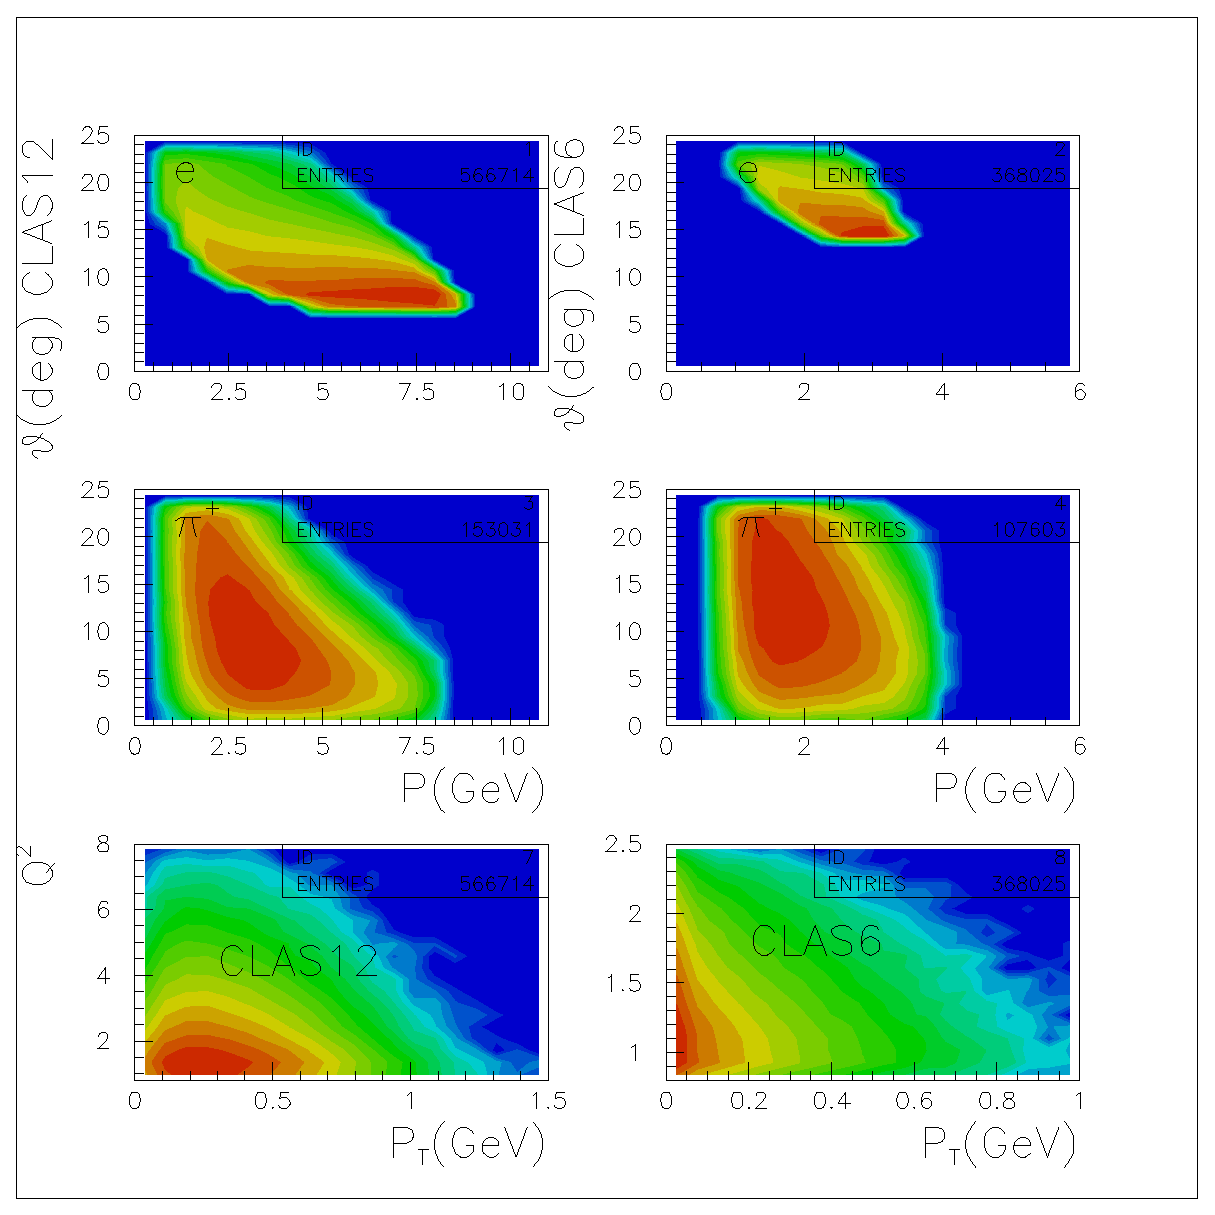
\epsfig{file=sidistrans.eps,width=14.0cm,height=8cm}
\vskip-0.2cm
\caption{\small{Kinematic coverage with the transversely polarized target 
(electron angles below 22.5$^\circ$).  The plots on the left show (top
to bottom) $\theta_e$ vs. $p_e$, $\theta_{\pi}$ vs. $p_{\pi}$, and $Q^2$ vs. 
$p_t$ for {\tt CLAS12}.  The plots on the right are the same but for
{\tt CLAS} at 6~GeV.}}
\label{fig:sidistrans}
\end{center}
\end{figure}
%%%%%%%%%%%%%%%%%%%%%%%%%%%%%%%%%%%%%%%%%%%%%%%%%%%%%%%%%%%%%%%%%%%%%%%%%%

\subsection{Transversely Polarized HD Frozen-Spin Target}

The magnetic holding fields accompanying transversely polarized targets can 
deflect an electron beam and create challenging background conditions.  A 
magnetic chicane can be installed upstream of the target and arranged in such 
a way that the target's magnetic field bends the electron beam back on axis. 
However, bremsstrahlung created in the target material will be peaked along 
the direction of the incoming electrons, which will then be at several 
degrees to the detector axis.  Generally, one can arrange to have either the 
electron beam or the target bremsstrahlung centered at 0$^\circ$, but not 
both.  A transversely polarized target in a frozen-spin state that requires 
only small holding fields would greatly mitigate such background problems. 
Problems associated with beam deflection are virtually eliminated by the 
small holding fields, and this potentially allows the target to be located in 
the center of the detector, thus dramatically increasing the acceptance.  In 
addition, the target has almost no dilution. The only unpolarizable nucleons 
are associated with the target cell and these can be sampled and subtracted 
in conventionally empty-cell measurements.  At the same time, the low $Z$
of the target material results in a long radiation length and comparatively 
few bremsstrahlung photons. 

The HDice target developed at LEGS in Brookhaven and now migrating from BNL 
to JLab, has been used successfully in photon beam experiments.  The factors 
affecting the target polarization are complex and intertwined; a direct test 
of the performance of polarized HD with electrons is essential.  This will 
be carried out during the course of the E06-101 run with {\tt CLAS}.

At BNL, HD target polarizations of 60\% $H$ and 35\% $D$ have been achieved 
in photon experiments with spin-relaxation times in excess of a year, and 
polarizations are expected to be higher with the smaller diameter cells 
that will be used at JLab. The deuterium polarization is particularly stable; 
spin-relaxation times of 2~months have been measured with only a 0.01~T 
holding field at 0.2 K. The projected $D$ decay time for a 0.04~T saddle coil,
0.12~m in length ($\int B \times  dL$ = 0.005~T-m), is $\sim$7 months.  
Comparable $H$ relaxation times require higher fields, but should be possible 
with $\int B \times dL$ = 0.050~T-m, which is still about 30 times less than 
a dynamically polarized ammonia target.  The beam heating expected from 5~nA 
of 10~GeV electrons traversing a 2-cm $HD$ target is $\sim$5~mW (as calculated 
with GEANT).  This is about the cooling power of the existing BNL 
In-Beam-Cryostat (IBC) at 0.5~K, and will be significantly increased in the 
{\tt CLAS}-IBC now under design for E06-101.  Beam heating is considerably 
less in $HD$, as compared to butanol, due to the lower $Z$ of the target 
material and, unlike butanol, $HD$ relaxation times are not such strong 
functions of temperature, so long life-times are achievable up to about 0.7~K.

Free radicals generated by electron bremsstrahlung will have randomly 
oriented polarizations.   While their absolute number is small, they can 
generate polarization sinks within the target if the spin-diffusion time is 
short. This time constant has been indirectly measured at BNL by using RF 
waves to punch a local polarization hole within a highly polarized target.  
The rate at which this hole heals after the RF power is lowered reflects the 
in-diffusion of spin from other regions of the target. At 2~K, this measured 
spin-diffusion is $\sim$1 day for $H$, but unmeasurably long for $D$ (greater 
than a year).  Whether or not the $H$ performance improves at lower 
temperatures is a matter for further study, but the extremely slow 
spin-diffusion for $D$ already suggests that frozen-spin $HD$ could maintain 
its deuterium polarization during electron experiments.  Frozen-spin HDice 
may provide an attractive alternative for electron experiments with at least 
transversely polarized deuterons in {\tt CLAS12}.

\section{The BoNuS Radial Time Projection Chamber}

The BoNuS experiment needed to detect very low-momentum recoil protons at
backward scattering angles used as a tag on quasi-free electron-neutron 
scattering from a deuterium target.  For that experiment, a radial time 
projection chamber (RTPC), surrounding an integrated thin-walled target gas 
cell, was built. This detector is going to be used for the conditionally 
approved experiment PR12-06-113, using the upgraded 11~GeV electron beam and 
{\tt CLAS12}, and can be used for other experiments with other target gases 
as well.

The RTPC will be placed inside the central detector solenoid magnet,
which will provide the analyzing magnetic field for the momentum 
determination via the track curvature of scattered charged particles.

The 283-mm long, thin-walled Kapton target tube can contain up to 7~atm of 
target gas, like deuterium, and is surrounded by the radial time projection 
chamber.  The sensitive drift region of the 200-mm long RTPC is an annulus 
with an inner radius of 30~mm and an outer radius of 60~mm.  Materials 
between the target gas cell and the sensitive detector volume are minimized 
to prevent energy loss of the scattered particles and to minimize the 
interaction of background particles.  These background particles are mostly 
M{\o}ller electrons forced into helical trajectories along the beam axis.

The amplification of the drifting electrons is achieved by three layers of 
gas electron multiplier (GEM) foils at radii of 60, 63, and 66~mm.  This is 
surrounded by a cylindrical readout surface at a radius of 69~mm. 

The resulting detector consists of two similar half-cylinder units that
are mated together on either side of the central beam axis.  Axial
mechanical structures fit within a $\pm$16$^\circ$ wedge along the top
and bottom of the assembly, as shown in Fig.~\ref{fig:prod_schem_expl}.
All of the structural components are light-weight and self-supporting.
These parts nest together to form the final detector module. 

%%%%%%%%%%%%%%%%%%%%%%%%%%%%%%%%%%%%%%%%%%%%%%%%%%%%%%%%%%%%%%%%%%%%%%%%%%
\begin{figure}[htbp]
\center{\epsfig{figure=DOUB_PHOTO_SCHEM.eps,width=14cm}}
\caption{\small{Schematic diagram and photograph of the BONUS RTPC. 
a)~Cross-section view through the center of the detector.  b)~Photograph of 
the left module with the readout pad board removed.}}
\label{fig:prod_schem_expl}
\end{figure}
%%%%%%%%%%%%%%%%%%%%%%%%%%%%%%%%%%%%%%%%%%%%%%%%%%%%%%%%%%%%%%%%%%%%%%%%%%

Gas electron multipliers are 50-$\mu$m thick polyimide foils coated on both 
sides with a 5~$\mu$m copper layer, and punctured with 70~$\mu$m holes. The 
distance between these holes is about 140~$\mu$m.  By applying a voltage in 
the range of 200~V to 300~V across the two copper layers, a very high 
electric field is formed inside the holes.  Electrons drifting towards the 
GEM foil produce an avalanche of secondary electrons when captured and 
accelerated through the holes.  The gain in each GEM is of the order of 100.
The electrons drift to the next GEM foil, and after passing through three GEM 
foils, the resulting electron pulse is detected on the readout plane.  The 
three GEM support frames were dimensioned such that identical GEM foils of 
an active area of 200~mm $\times$ 170~mm could be used throughout.  The 
voltage was chosen such that the RTPC was insensitive to minimum ionizing 
particles, such as electrons and most pions, but had an excellent detection 
efficiency for highly ionizing recoil protons.

The outermost cylindrical layer of the detector is the readout board made out
of a flexible polyimide substrate. It carries gold-plated conductive pads
on the inner surface with a pattern of 4.45~mm $\times$ 5~mm, as shown
in Fig.~\ref{fig:padpat}. The pads are connected by closed vias to the
outer surface on which groups of 16 pads are traced to a common connector,
carrying 16-channel preamplifier cards.

%%%%%%%%%%%%%%%%%%%%%%%%%%%%%%%%%%%%%%%%%%%%%%%%%%%%%%%%%%%%%%%%%%%%%%%%%%
\begin{figure}[htbp]
\vspace{6.5cm}
\special{psfile=brickpads4nim.eps hscale=80 vscale=80 hoffset=80 voffset=-50}
\caption{\small{Pad geometry in the production RTPC. There are 40 rows and
40 columns of pads. Pad rows (along the cylindrical axis) are offset from 
one another to improve the track resolution.}}
\label{fig:padpat}
\end{figure}
%%%%%%%%%%%%%%%%%%%%%%%%%%%%%%%%%%%%%%%%%%%%%%%%%%%%%%%%%%%%%%%%%%%%%%%%%%

The signals are inverted on these cards and transmitted via 6-m long cables 
to a low-impedance receiver circuit, feeding the positive signals into the 
readout electronics developed at CERN for the TPC of the ALICE experiment, 
under construction at the Large Hadron Collider for heavy-ion collisions.
Each readout card provides 128 channels of pre-amplification, digitization
via a 10-bit ADC, signal correction circuits, and a pipeline buffer for 
eight events.  Each event contains the signals of all pads integrated over 
a selectable time interval in the range of 100~ns for a period of up to 100 
intervals, in this case 10~$\mu$s.  Of the 100 intervals, up to 15 can be 
before the arrival of the trigger from {\tt CLAS}.

Signals below preset thresholds, taking dynamically calculated and preset 
pedestals into account, are suppressed in the data stream to decrease the 
data volume, for an increase of the event rate. Thirteen readout cards are 
needed to read out one half-cylinder of the detector.  They are grouped 
into one crate, controlled by one readout control card (RCU).  Two crates 
are needed to read out the whole RTPC.  Each RCU is connected at present 
via USB 2.0 to a VME based Motorola crate controller, forming the standard 
readout unit in the {\tt CLAS} data acquisition system.

\section{Ring Imaging {\v C}erenkov for {\tt CLAS12}}

The particle identification system (PID) of the {\tt CLAS12} forward detector 
is based on the information from the Forward Time-of-Flight counters (FTOF), 
the Low Threshold {\v C}erenkov Counters (LTCC), the High Threshold 
{\v C}erenkov Counters (HTCC), the Pre-shower Calorimeters (PCAL), and the 
Electromagnetic Calorimeters (EC). The combination of the LTCC, HTCC, and EC 
counters will allow a good separation between electrons and pions for momenta 
up to 5~GeV.  The performance of the {\tt CLAS12} PID system for charged 
hadrons is summarized in Fig.~\ref{fig:pid}.  Green indicates good PID and
yellow shows where there are limitations of the system and how far it can be 
pushed. The case of the separation between pions and kaons for momenta  
between 2.6 and 5~GeV is a good example.  By combining the information from 
the FTOF and LTCC, one can get some kind of separation between kaons and 
pions, although not very satisfactory.  Red indicates the absolute limitation 
of {\tt CLAS12} PID in the high momentum range above 5~GeV.

Good PID is a crucial element in the success of any experimental program as 
important and as diverse and as rich in physics as the one planned for 
{\tt CLAS12}.  Good kaon identification over the entire momentum range is 
very important for the polarized and unpolarized semi-inclusive deep inelastic
measurements, such as the contribution of the strange sea to the nucleon spin 
and the transversity measurements for kaons. The study of hadronization will 
also benefit tremendously from very good PID.

%%%%%%%%%%%%%%%%%%%%%%%%%%%%%%%%%%%%%%%%%%%%%%%%%%%%%%%%%%%%%%%%%%%%%%%%%%
\begin{figure}
\epsfxsize=12cm
\epsfysize=8cm
\centerline{\epsfbox{clas12-pid-n.ps}}
\vspace{-0.3 cm}
\caption{\small{Summary of the performance of the {\tt CLAS12} PID system 
for charged hadrons.}}
\label{fig:pid}
\end{figure}
%%%%%%%%%%%%%%%%%%%%%%%%%%%%%%%%%%%%%%%%%%%%%%%%%%%%%%%%%%%%%%%%%%%%%%%%%%

To improve the {\tt CLAS12} PID system from good to excellent, one needs to 
build a ring imaging {\v C}erenkov (RICH) detector.  Due to space 
limitations, the only place where this detector would fit is the LTCC 
location.  One can think of exchanging one or more sectors of LTCC by 
a RICH detector.  The design of the RICH detector~\cite{Akopov:2000qi} of 
HERMES experiment would be a good choice for {\tt CLAS12}.  It is a dual 
radiator RICH detector that uses a clear aerogel in combination with a heavy 
gas, C$_{4}$F$_{10}$. It can provide a clean separation of pions, kaons, and 
protons in the desired momentum region. The {\v C}erenkov angles produced by 
the combination of the aerogel and the C$_{4}$F$_{10}$ gas for pions, kaons,
and protons are plotted in Fig.~\ref{fig:ccangle}. The corresponding threshold 
momenta are listed in Table~\ref{tab:threshold}.

%%%%%%%%%%%%%%%%%%%%%%%%%%%%%%%%%%%%%%%%%%%%%%%%%%%%%%%%%%%%%%%%%%%%%%%%%%
\begin{figure}
\epsfxsize=10cm
\epsfysize=9cm
\centerline{\epsfbox{RICH-ang.ps}}
\vspace{-0.3 cm}
\caption{\small{The {\v C}erenkov angle vs. hadron momentum for the 
aerogel and the C$_{4}$F$_{10}$ gas radiators.}}
\label{fig:ccangle}
\end{figure}
%%%%%%%%%%%%%%%%%%%%%%%%%%%%%%%%%%%%%%%%%%%%%%%%%%%%%%%%%%%%%%%%%%%%%%%%%%

%%%%%%%%%%%%%%%%%%%%%%%%%%%%%%%%%%%%%%%%%%%%%%%%%%%%%%%%%%%%%%%%%%%%%%%%%%
\begin{table}
\begin{center}
\begin{tabular}{|c|c|c|} \hline 
       & Aerogel & $C_{4}F_{10}$ \\ \hline                        
$n$    & 1.0304  & 1.00137 \\ \hline 
Pions  & 0.6 GeV & 2.7 GeV \\ \hline 
Kaons  & 2.0 GeV & 9.4 GeV \\ \hline 
Protons& 3.8 GeV & 17.9 GeV \\ \hline 
\end{tabular}
\end{center}
\caption{\small{{\v C}erenkov light thresholds for pions, kaons, and protons 
for the aerogel and C$_{4}$F$_{10}$ gas radiators.}}
\label{tab:threshold}
\end{table}
%%%%%%%%%%%%%%%%%%%%%%%%%%%%%%%%%%%%%%%%%%%%%%%%%%%%%%%%%%%%%%%%%%%%%%%%%%

\section{Central Electromagnetic Calorimeter}

\subsection{Overview}

The central electromagnetic calorimeter is an essential part of the 
{\tt CLAS12} central detector.  It covers detection angles in the polar 
range from $40^\circ \leq \theta \leq 135^\circ$, and in almost the entire 
azimuthal range.  It is designed for the reconstruction of $\pi^0$ and 
$\eta$ mesons by their neutral decays, therefore, for the detection of 
multi-$\gamma$ events.  The design parameters are defined to meet an 
operational luminosity of $L \sim 10^{35}$~cm$^{-2}$s$^{-1}$.  The following 
sections describe the technical requirements, the detailed design concept, 
and the estimates for the calorimeter performance.

\subsection{Requirements}

The compact structure of the entire central detector, which is mounted 
inside a superconducting solenoid with a strong magnetic field, determines 
the basic parameters of the calorimeter.  The available radial space for 
the calorimeter material inside the magnet is limited to $\sim 10$~cm.  The 
calorimeter must provide adequate energy and spatial resolutions to cleanly 
identify $\pi^0$ and $\eta$ events.  The typical energies of decay photons, 
produced at large angles ($>40^\circ$) and at beam energies of 12~GeV, are 
up to $E_\gamma \sim 1$~GeV.  Reasonable energy resolution with these size 
restrictions can only be achieved if very dense materials are used, and at 
the same time, the sampling ratio and homogeneity of the calorimeter are 
reasonably high. The $\pi^0$ and $\eta$ mass resolutions are functions of 
the energy and angular resolutions.  

In order to provide sufficient mass resolution, i.e. 
$\delta m \sim 1/3(m/2)$, for $\pi^0$ and $\eta$ mesons, it is 
necessary to have energy resolutions of about $\sigma/E_\gamma \leq 6\%$ at 
$E_\gamma \sim 1$~GeV and angular resolutions of 
$\delta \theta \sim 0.8^\circ -1.4^\circ$.  The angular resolution depends 
on the number of channels used to measure $\phi$ and $\theta$. Taking into 
account that transverse shower dimensions are expected to be of  
$\sim$20~mm ($\sim$80\% containment), the lower limit of the angular 
resolution is estimated to be $\delta \theta \sim 1^\circ$ .  To detect 
$\pi^0$s of the lowest energy, the calorimeter must provide an energy 
threshold of about $\sim$50~MeV.  To prevent major shower energy leakages 
for photons at angles close to $\theta = 90^\circ$ (worst case), the 
calorimeter should be  $\sim$10 - 11 radiation lengths deep at 
$E_\gamma$ = 1~GeV.  Table~\ref{parameters} shows the main design parameters 
of the Central Calorimeter.

%%%%%%%%%%%%%%%%%%%%%%%%%%%%%%%%%%%%%%%%%%%%%%%%%%%%%%%%%%%%%%%%%%%%%%%%%%
\begin{table}
\begin{center}
\begin{tabular}{||l|l||}  \hline\hline
Total Radiation Lengths            & 10 - 12 \\ \hline 
Radial Space (radial thickness)    & $\sim$ 10 cm \\ \hline
Energy Resolution                  & $\approx 6\%/\sqrt{E}$  \\ \hline
Angular Resolution, $\delta \theta = \delta \phi$ & $\sim 1^\circ$ \\ \hline
Timing Resolution, $\delta t$      & few ns \\ \hline
Energy Threshold, $E^{min}_\gamma$ & $\leq$ 50 MeV \\ \hline\hline 
\end{tabular}
\caption{\small{Central electromagnetic calorimeter design parameters.}}
\label{parameters}
\end{center}
\end{table}
%%%%%%%%%%%%%%%%%%%%%%%%%%%%%%%%%%%%%%%%%%%%%%%%%%%%%%%%%%%%%%%%%%%%%%%%%%

\subsubsection{Scintillating Fiber/Tungsten Powder Calorimeter Design}

The overall view and basic dimensions of the cylindrical central calorimeter 
mounted inside the solenoid magnet are shown in Fig.~\ref{yrs1}.  Dense 
tungsten metal powder is used as the absorber.  Thin plastic scintillating 
fibers run in the direction parallel to the beam and are read out from the 
upstream end as shown in Fig.~\ref{yrs2}.  The fibers are grouped into 
groups of equal size.  Each group of fibers, which cover an azimuthal angle 
range $\Delta \phi \approx \pm 0.6^\circ$, go to a single photo-multiplier 
tube that provides energy, $\phi$, and timing information.  In the radial 
direction, there are one or two layers of fibers (see Fig.~\ref{yrs3}) that
all bend at the same radius with both ends running out of the sensitive volume 
as shown in Fig.~\ref{yrs4}. This circular layer of grouped fibers provides 
independent measurements of the polar angle $\theta$ of the shower. To have 
resolutions of $\delta \theta \approx 1^\circ$, there will be a total of 
about 50 channels per polar angle measurement.  To allow all the fibers to 
run through the main volume (see Fig.~\ref{yrs4}), there is a narrow gap 
not wider than 5~mm along the beam direction for readout purposes.  This gap 
produces only a small reduction in the angular acceptance of the calorimeter 
(about 1-2\%). 

%%%%%%%%%%%%%%%%%%%%%%%%%%%%%%%%%%%%%%%%%%%%%%%%%%%%%%%%%%%%%%%%%%%%%%%%%%
\begin{figure}[tb]
\vspace{8.0cm} 
\special{psfile=cent_cal_sep.ps hscale=45 vscale=45 hoffset=95 voffset=-70}
\caption{\small{A perspective view of the central electromagnetic 
calorimeter inside the solenoid magnet.}}
\label{yrs1}
\end{figure}
%%%%%%%%%%%%%%%%%%%%%%%%%%%%%%%%%%%%%%%%%%%%%%%%%%%%%%%%%%%%%%%%%%%%%%%%%%

The implementation for this topology of the calorimeter with two sets of 
scintillating fibers embedded within essentially the same sensitive volume,
is only possible because of the powder technology -- the volume is filled 
by loose metal powder. Since the so-called ``green density'' of the 
tungsten powder to be used as absorber is of about $12 \pm 0.2$~g/cm$^3$, 
the entire structure becomes very efficient, especially in providing high 
sampling ratios with fibers as thin as 0.5 - 0.75~mm (or even smaller 
diameters), with no air gaps between the fibers and absorber.  This 
particular feature allows matching two requirements, having sufficient 
energy resolution and small overall dimensions at the same time.

%%%%%%%%%%%%%%%%%%%%%%%%%%%%%%%%%%%%%%%%%%%%%%%%%%%%%%%%%%%%%%%%%%%%%%%%%%
\begin{figure}
\vspace{6.7cm} 
\special{psfile=cent_cal_sep2.ps hscale=45 vscale=45 hoffset=95 voffset=-90}
\caption{\small{Central calorimeter. The tungsten powder volume and some of 
the axial readout fibers are shown at the left.  Some of the radial fibers 
are indicated on the right side.  The radial fibers are brought to the 
readout end through a slot at the bottom of the calorimeter.}}
\label{yrs2}
\end{figure}
%%%%%%%%%%%%%%%%%%%%%%%%%%%%%%%%%%%%%%%%%%%%%%%%%%%%%%%%%%%%%%%%%%%%%%%%%%

%%%%%%%%%%%%%%%%%%%%%%%%%%%%%%%%%%%%%%%%%%%%%%%%%%%%%%%%%%%%%%%%%%%%%%%%%%
\begin{figure}
\vspace{7.8cm} 
\special{psfile=cent_cal_aug3.ps hscale=25 vscale=25 hoffset=190 voffset=50}
\caption{\small{Central Calorimeter. The radial fibers are interleaved with 
the axial fibers. They provide shower position information along the beam 
direction. Since they are not used for the energy measurement, only a few 
layers are needed to provide the position information.}}
\label{yrs3}
\end{figure}
%%%%%%%%%%%%%%%%%%%%%%%%%%%%%%%%%%%%%%%%%%%%%%%%%%%%%%%%%%%%%%%%%%%%%%%%%%

%%%%%%%%%%%%%%%%%%%%%%%%%%%%%%%%%%%%%%%%%%%%%%%%%%%%%%%%%%%%%%%%%%%%%%%%%%
\begin{figure}
\vspace{8.0cm} 
\special{psfile=cent_cal_aug4.ps hscale=25 vscale=25 hoffset=160 voffset=-20 angle=0}
\caption{\small{Central Calorimeter: radial fibers read out (detail) in the 
slot at the bottom of the calorimeter.}}
\label{yrs4}
\end{figure}
%%%%%%%%%%%%%%%%%%%%%%%%%%%%%%%%%%%%%%%%%%%%%%%%%%%%%%%%%%%%%%%%%%%%%%%%%%

\subsubsection{Expected Performance}

To estimate the calorimeter response, one can use parameterizations based 
on simulations and previous calorimeter data. We have used parameterizations 
during the initial design phase for a fast estimation of the basic 
dimensions and characteristics of the calorimeter.  The containment of the 
shower is parameterized using~\cite{Fab85}:

\begin{equation}
L (98\%) = 2.5*[\log(\frac{E}{\epsilon}) + 1.2] \times X_o~{\rm (cm)}.
\end{equation}

Here, $L$ gives the length in centimeters that contains about 98\% of the 
energy of the shower.  $E$ is the energy of the incoming photon, $\epsilon$ 
the critical energy of the material, and $X_o$ is the radiation length of 
the mix in centimeters.  The material in the calorimeter is a mix of 
tungsten powder and scintillating plastic (Polystyrene) fibers.  The 
radiation length for the mix ($X_o$) that contains a fraction $y$ of 
scintillating plastic per volume and a fraction $(1-y)$ of tungsten powder 
absorber, is obtained using:

\begin{equation}
\frac{1}{X_o} = \frac{y}{X_{Sci}} + \frac{(1-y)}{X_{Powder}}.
\end{equation} 

For the powder with a fraction $x$ of the pure tungsten, the total
thickness in radiation lengths is given by $X_{Powder}=X_{Pure Tungsten}/x$.
The critical energy of the mix is obtained using: 
 
\begin{equation}
\epsilon = y \epsilon_{Sci} + (1-y) \epsilon_{Powder}.
\end{equation}

The results are shown in Fig.~\ref{errlon}.  The values of $L$ are 
plotted versus the fraction of scintillating plastic by volume for three 
values of the powder density: $x$=0.62 (loose powder), $x$=0.8 (cold 
pressed density), and $x$=1.0 (pure tungsten).  One can see that if the 
radial thickness of the calorimeter, using loose powder at $x$=0.62, is 
limited by $\sim$10~cm, then the fraction of scintillating plastic should 
not exceed $\sim$35\% per volume.

%%%%%%%%%%%%%%%%%%%%%%%%%%%%%%%%%%%%%%%%%%%%%%%%%%%%%%%%%%%%%%%%%%%%%%%%%%
\begin{figure}
\vspace{9.0cm} 
\special{psfile=errlon.eps hscale=45 vscale=45 hoffset=115 voffset=0}
\caption{\small{Containment vs. fraction of plastic for the central
calorimeter.}}
\label{errlon}
\end{figure}
%%%%%%%%%%%%%%%%%%%%%%%%%%%%%%%%%%%%%%%%%%%%%%%%%%%%%%%%%%%%%%%%%%%%%%%%%%

The other important figure-of-merit is provided by the sampling errors in 
the energy measurements.  For a given material ($x$=0.62), these sampling 
errors are a function of the fraction of scintillating plastic in the 
calorimeter $y$ (sampling fraction) and the diameter of the fibers $\phi$ 
(sampling frequency).  The corresponding parameterization for the sampling 
errors is given by~\cite{Wig20}: 

\begin{equation}
{\frac{\sigma}{E}}_{sampling} = 0.02 \sqrt{\frac{\phi(mm)}{f_{sampl}}},
\end{equation}

\noindent
where $f_{sampl}$ is the sampling ratio for minimum ionizing particles,
and is calculated using:

\begin{equation}
f_{sampl} = \frac{1}{1+\frac{(1-y)}{y} x \frac{dE_{W}}{dE_{Sci}}}.
\end{equation}

\noindent
Here, $dE_{W}$ and $dE_{Sci}$ are the energy depositions by minimum 
ionizing particles in 1~cm of tungsten (22.1~MeV/cm) and polystyrene 
(2.0~MeV/cm), respectively.
 
Fig.~\ref{errvol6} shows the sampling errors versus the fraction of 
scintillating plastic by volume for four different fiber diameters (0.25, 
0.5, 0.75, and 1~mm), at a powder density of $x$=0.62.  One can see that 
for an absorber density of 11.8~g/cm$^3$ ($x$=0.62), a tungsten powder 
based sampling calorimeter built with fibers of 0.5~mm in diameter and 
with a fraction of scintillating fibers of $\sim$35\% per volume can reach 
energy resolutions better than $\sim$6\% at 1~GeV energies.  This 
resolution is similar to that obtained by the KLOE~\cite{Ant96} and 
JETSET~\cite{Hert90} calorimeters using a larger number of scintillating 
fibers.  In Fig.~\ref{errvol6}, the value of $\sigma/E$ obtained by the KLOE 
collaboration~\cite{Ant96} with a sampling calorimeter of 23~cm radial 
thickness built at $y$=0.5 using lead absorbers and 1~mm polystyrene fibers
is also shown.

%%%%%%%%%%%%%%%%%%%%%%%%%%%%%%%%%%%%%%%%%%%%%%%%%%%%%%%%%%%%%%%%%%%%%%%%%%
\begin{figure}
\vspace{9.0cm} 
\special{psfile=errvol6.eps hscale=45 vscale=45 hoffset=115 voffset=10}
\caption{\small{Sampling errors vs. fraction of plastic for the central
calorimeter.}}
\label{errvol6}
\end{figure}
%%%%%%%%%%%%%%%%%%%%%%%%%%%%%%%%%%%%%%%%%%%%%%%%%%%%%%%%%%%%%%%%%%%%%%%%%%

\subsubsection{Prototyping and Simulations}

The proposed sampling calorimeter is to be build using a new calorimetry 
construction technology.  There are open questions that need to be answered, 
although some initial tests already have been successfully carried out.

\begin{itemize}
 
\item An important test will be to establish the more efficient assembly 
procedure when fibers having different directions and shapes are installed 
in the same volume.
 
\item We need to explore the limits on sampling frequencies available with 
this technique, especially with fibers of small diameters. Small fibers 
($\sim$0.25~mm) cannot be used with other techniques (grooving), unless one 
allows lots of air gaps or glue. Also the technical limits for 
sampling ratios with tungsten powder radiator have to be found. First tests 
have shown that designs are possible with a sampling ratio $\sim$17\% and 
340 polystyrene fibers of 0.5~mm in diameter using loose tungsten powder. 
A density of not less than 11.8~g/cm$^3$ can be achieved.  Further tests are 
in progress.

\item The main features of the calorimeter with a given realistic geometry 
need detailed simulation (i.e, using GEANT). This simulation will define 
the expected energy and angular resolutions to be compared with experimental 
test values that can be used in planning of physics experiments.

\item A prototype consisting of 12 channels is currently being designed and 
built to examine all basic properties of the calorimeter. The final goal is 
to test the calorimeter in a photon or electron beam in the very near 
future.  This first full prototype will have $\sim$10~cm of thickness 
($\sim$11 radiation lengths) with a fraction of plastic of 35\% by volume 
using polystyrene fibers of 0.75~mm in diameter.

\end{itemize}

%\bibliography{../bonus/bonus,../rich/rich,../centralec/centralec}



